\chapter{NoSQL}
\begin{nota}
      In quest capitolo non si vuole sostenere che i database NoSQL siano
      migliori di quelli relazionali. I database NoSQL sono un'alternativa
      ai database relazionali e non sempre sono la scelta migliore. Per ogni
      applicazione è necessario valutare quale sia la scelta migliore.
\end{nota}
Fino a questo momento abbiamo utilizzato database relazionali per gestire le
nostre applicazioni. Tuttavia, i database relazionali non sono l'unica
opzione disponibile. In questo capitolo, esploreremo un'alternativa ai
database relazionali: i database NoSQL.
\section*{Use Cases}
\subsection*{Crypto}
Iniziamo analizzando uno Use Case. Un cliente vuole salvare dati legati alle
crypto che vengono forniti da un API. Con le conoscenze conseguite fino a questo
momento, salveremo tutto su una tabella di un DBMS relazionale dove si hanno 5 colonne:
\begin{itemize}
      \item id
      \item Simbolo
      \item Prezzo\_USD
      \item Prezzo\_EUR
      \item Data
\end{itemize}
Nel caso in cui nella risposta fossero presenti informazioni aggiuntive o nel caso
in cui si volessero salvare informazioni aggiuntive, si dovrebbe modificare la
tabella. Questo si può osservare soprattutto quando si hanno risposte molto
complesse, perché salvare dati in molteplici tabelle significa per ottenere
l'informazione intera si devono fare molte join, questo comporta un rallentamento
delle prestazioni.

Una soluzione per ridurre il numero di join è quello di duplicare i dati, il
problema è che i dati che si duplicano devono essere consistenti. In aggiunta
posso ridurre le tabelle unendole creando una grande tabella che può essere
frammentata a livello fisico, il problema di questa soluzione è che si vanno a
inserire un elevato numero di valori \texttt{null}.
\subsection*{Social network}
Un altro caso d'uso è il social network in cui si vuole salvare la relazione di
amicizia tra profili, il problema è che se si avessero 1M di utenti, ciascuno con
100 amici, allora la tabella amicizia diventa 100M di record. Troppa complessità
soprattutto per una tabella che verrà usata spesso con delle join.

Il DB relazionali non sono in grado di modellare efficientemente i contesti applicativi
con volumi molto significativi di dati.
\section{Introduzione}
Da questo use case possiamo osservare che il modello relazionale presenta dei
limiti nella gestione dei dati:
\begin{itemize}
      \item Si ha uno svantaggio nel salvare di dati poco omogenei, questo è dovuto
            principalmente alla rigidità dello schema. In quanto prima di poter
            inserire i dati, è necessario definire uno schema.
      \item Si ha uno svantaggio in relazione al paradigma di programmazione che
            viene usato (Programmazione a oggetti). Questo obbliga a utilizzare
            un ORM per mappare i dati del database relazionale con gli oggetti
            del linguaggio di programmazione.
\end{itemize}
Inoltre, essendo le risposte delle API solitamente in formato JSON, si ha un
ulteriore svantaggio in quanto si deve fare un parsing della risposta per
poterla salvare nel database relazionale.

I database NoSQL sono nati con lo scopo di risolvere alcuni problemi di quelli
relazionali come la scalabilità e la flessibilità. Inoltre, le assunzioni che
si trovano dietro i database relazionali non sono sempre adatte per tutti i
casi d'uso.

Con questo non vogliamo dire che i database NoSQL siano migliori di quelli
relazionali, ma che sono un'alternativa ai database relazionali. Per ogni
applicazione è necessario valutare quale sia la scelta migliore. Di seguito
elenchiamo alcuni motivi per cui utilizzare i database relazionali:
\begin{itemize}
      \item SQL è semplice.
      \item Molto rigido
      \item Vincoli nel database allora le app possono non fare i controlli
      \item ipotesi di mondo chiuso: tutto quello che serve è nel database, se non
            lo so devo inserire il valore \texttt{null}.
      \item Tecnologia stabile e funzionante che alle spalle anni di ricerca e
            sviluppo.
      \item Sono valide le proprietà ACID, molto utili in contesti in cui si
            hanno transazioni.
\end{itemize}
È corretto presentare anche gli svantaggi dei database relazionali:
\begin{itemize}
      \item Modificare una tabella nella quale sono già presenti dei valori è molto
            complicato.
      \item Assunzione mondo chiuso: può risultare troppo pesante in determinate
            situazioni.
      \item Il concetto di minimizzare le ripetizioni dei valori implica la necessità
            di effettuare molte join per ottenere l'informazione desiderata.
      \item Si ha un mapping un attributo ha un valore.
      \item Non è compatibile con i linguaggi di programmazione ad oggetti.
      \item Presenta delle difficoltà nella gestione dei self-join.
      \item È difficilmente scalabile.
\end{itemize}
\begin{nota}
      Il termine NoSQL significa \textit{Not Only SQL}.
\end{nota}
Una caratteristica comune dei database NoSQL è che sono \textbf{schema-free} o
\textbf{schema-less}. Questo significa che non è necessario definire uno schema
prima di poter inserire i dati. L'inserimento dei dati implica per quel dato lo
schema associato, il successivo inserimento di un dato può avere uno schema diverso.

% Presa da internet la definizione
Oltre a ciò, per questi database vale il teorema CAP, che afferma che è
impossibile per un sistema distribuito garantire contemporaneamente le seguenti
tre proprietà:
\begin{itemize}
      \item \textbf{Consistency}: tutti i nodi vedono gli stessi dati allo stesso
            tempo.
      \item \textbf{Availability}: ogni richiesta riceve una risposta, anche in
            presenza di guasti.
      \item \textbf{Partition tolerance}: il sistema continua a funzionare anche
            se alcune parti del sistema non sono disponibili.
\end{itemize}

Mentre nei database relazionali avevamo le transazioni ACID, nei database NoSQL
abbiamo le transazioni BASE, che stanno per:
\begin{itemize}
      \item \textbf{Basically Available}: il sistema è sempre disponibile.
      \item \textbf{Soft state}: lo stato del sistema può cambiare anche senza
            input.
      \item \textbf{Eventual consistency}: il sistema diventerà consistente in un
            certo momento.
\end{itemize}

Inoltre, a differenza dei database relazionali, i database NoSQL si basano su
un'assunzione di mondo aperto, ovvero viene inserito solo quello che conosco se
mi mancano delle informazioni non le metto.

Si è passati dal progettare le architetture in modo da essere più specifiche
per l'applicazione, il contrario di come si faceva una volta: progettazione generalista.
\section{Tipi di database NoSQL}
Esistono diverse tipologie di database NoSQL, ognuna con le proprie caratteristiche
e i propri casi d'uso. Possiamo dire che più è semplice il modello, più è facile
scalarlo. Nella figura \ref{fig:tipi_nosql} possiamo come si posizionano i
database NoSQL rispetto alla dimensione e complessità del modello.
\begin{figure}[!ht]
      \centering
      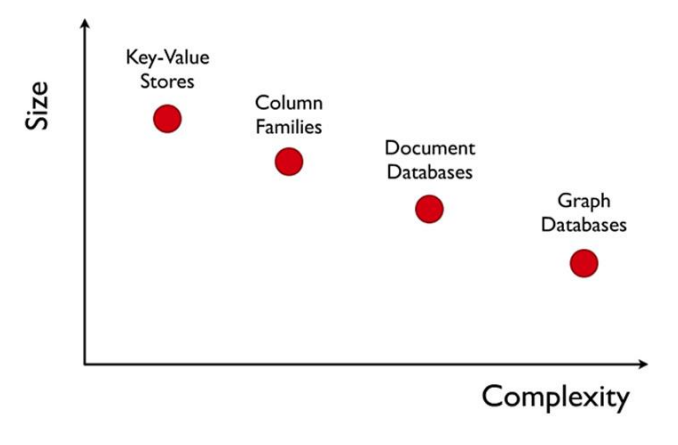
\includegraphics[scale=0.5]{./img/nosql/tipi_nosql.png}
      \caption{Tipi di database NoSQL}
      \label{fig:tipi_nosql}
\end{figure}
Rispetto questa rappresentazione possiamo posizionare il modello relazionale a metà
tra la complessità delle colonne e i documenti.
In questo corso vedremo i seguenti tipi di database NoSQL:
\begin{itemize}
      \item \textbf{Document-based}: i dati sono memorizzati in documenti, che
            possono essere in formato JSON, XML, BSON, YAML, etc.
      \item \textbf{Key-value}: i dati sono memorizzati in coppie chiave-valore.
      \item \textbf{Wide-column}: i dati sono memorizzati in colonne, simile ai
            database relazionali.
      \item \textbf{Graph-based}: i dati sono memorizzati in nodi e archi.
\end{itemize}
Una caratteristica che accomuna questi modelli è che tutti devono risolvere il
problema di mettere insieme i dati. Ad esempio, i database relazionali usano i join,
mentre i database document-based usano un unico documento.
\subsection{Key value}
I database key-value sono i più semplici tra i database NoSQL. In questi
database, i dati sono memorizzati come tabelle di hash dove la chiave punta a un
particolare valore. Si utilizzano le tabelle di hash per massimizzare le prestazioni
di lettura e scrittura.
\subsection{Wide column}
I database wide-column sono simili ai database relazionali, ma invece di
memorizzare i dati in righe, i dati sono memorizzati in colonne. Questo permette
di avere una maggiore flessibilità rispetto ai database relazionali. La chiave
punta a un insieme di colonne che può essere diverso per ogni riga.

\paragraph{HBASE}
HBase è un database wide-column che è stato ispirato da Google BigTable. In HBase
si ha una chiave che punta ad un insieme di valori che possono avere tipi differenti.

In questa struttura, possiamo definire delle \textbf{column family}, le quali
contengono più attributi che condividono delle informazioni. Il \textbf{qualifier} è
il nome dell'attributo all'interno di una column family. Ogni riga ha anche
un campo relativo al timestamp in cui è stata modificata.

L'utilizzo di timestamp fornisce un modo diverso per gestire le transazioni,
anche quelle distribuite, senza l'uso di lock. Questo metodo associa a ogni
transazione un timestamp, in modo che se due transazioni si sovrappongono,
possono essere risolte in base a tale valore.

In questa implementazione è possibile realizzare facilmente relazioni di tipo 1-n
nella stessa riga.
\paragraph{Cassandra}
Cassandra è un database wide-column che è stato realizzato da Facebook per gestire
la comunicazione con le mail.

Questo database si differenzia da HBase per il fatto si ha uno spazio delle chiavi,
il quale può essere visto come una tabella nel modello relazionale. Questo spazio
è suddiviso in column family, le quali sono differenti da quelle di HBase in quanto
la stessa chiave primaria può essere usata in più column family.

I valori che si trovano all'interno di una column family possono essere di tipo
diverso, inoltre, ogni riga ha un timestamp associato.

Quindi una column family equivale ad una \textit{tabella}, e si utilizza la chiave
primaria della riga per accedere ad un particolare dato di essa.

L'accesso viene effettuato specificando i seguenti campi:
\begin{itemize}
      \item \texttt{column family}
      \item \texttt{row key}
      \item \texttt{column name}
\end{itemize}
Per semplificare il passaggio da database relazionali a Cassandra, il query
language di Cassandra (CQL) è molto simile a SQL. Attraverso questo meccanismo
è possibile sviluppare un applicazione che è in grado di utilizzare sia database
relazionali che Cassandra senza apportare molte modifiche.

Un vantaggio dell'utilizzo di questo database è legato al fatto che ogni riga è
indipendente dalle altre. Quindi, in un contesto distribuito, è possibile frammentare
come si vuole il database senza dover fare join.
\subsection{Document based}
I database document-based permettono di memorizzare delle informazioni sotto
forma di documenti. Ognuno dei quali è identificato attraverso una chiave unica.
Tutte le operazioni di lettura e manipolazione dei dati avvengono all'interno
dei documenti stessi.
\paragraph{MongoDB}
MongoDB è un database document-based che memorizza i dati in documenti JSON.
Ogni documento è identificato da una chiave unica, chiamata \texttt{\_id}.

Possiamo immaginare la struttura di un file JSON come un albero, dove la radice
è la chiave \texttt{\_id} e i figli sono i campi del documento.

Questa tipologia permette di salvare i dati come si faceva negli schemi relazionali,
ovvero suddividendo le informazioni in diverse \textbf{collezioni}. Per fare ciò,
si utilizzano i \textbf{riferimenti} tra i documenti. Lo svantaggio di questa
soluzione è che si devono fare molte join per ottenere l'informazione desiderata.

Un'altra soluzione è quella di salvare i dati in un unico documento, sfruttando
l'embedding, in modo da evitare le join. Questo metodo è molto efficiente quando
si devono accedere alle informazioni più vicine alla radice, ma meno efficiente
quando si devono accedere alle foglie, si ha comunque un tempo di accesso minore
rispetto alle join.

Nei database document-based lo schema non è vincolante, in particolare, corrisponde
all'unione di tutti gli attributi e sotto-attributi del documento.

Vediamo ora un parallelismo tra i database relazionali e MongoDB:
\begin{itemize}
      \item \textbf{Database} $\rightarrow$ \textbf{Database}
      \item \textbf{Tabella} $\rightarrow$ \textbf{Collection}
      \item \textbf{Row} $\rightarrow$ \textbf{Document}
      \item \textbf{Column} $\rightarrow$ \textbf{Field}
      \item \textbf{Index} $\rightarrow$ \textbf{Index}
      \item \textbf{Join} $\rightarrow$ \textbf{Embedded document}
      \item \textbf{Foreign key} $\rightarrow$ \textbf{Reference}
      \item \textbf{Partition} $\rightarrow$ \textbf{Shard}
\end{itemize}
Le operazioni che si vogliono svolgere sulla base di dato vengono espresse
attraverso una notazione che ricorda quella della programmazione a oggetti, ovvero
attraverso la \textit{dot notation}. Inoltre, nelle operazioni tutti gli
operatori devono essere espressi in JSON. Questo permette di eliminare l'utilizzo
di framework come Hibernate per mappare gli oggetti sul database.
\begin{nota}
      Quando si devono caricare grandi quantità di dati è utile disabilitare
      l'ack che viene mandato per ogni operazione.
\end{nota}
Le query di modifica di un documento presentano degli oggetti JSON come
clausole, simile alla clausola \texttt{WHERE} delle query SQL. Oltre a questo
è possibile specificare di creare un documento nuovo nel caso non sia presente
quello che si vuole modificare.

Mongo permette di creare degli indici per velocizzare le operazioni.
\begin{esempio}
      Vediamo ora un esempio di parallelismo tra una query SQL e una per
      MongoDB:
\end{esempio}
Nelle interrogazioni, tutte le clausole sono specificate in \texttt{AND}, se si
vuole specificare in \texttt{OR} è necessario utilizzare il comando $\$or$ seguito
da una lista di oggetti JSON.

Nelle versioni successive è stato definito il concetto di \textbf{aggregation} e
di \textbf{pipeline}. Una pipeline è un comando che rappresenta una sequenza di 
operazioni che vengono eseguite in serie e possono essere usate per operazioni 
di analytics.

\subsection{Graph based}
I database graph-based memorizzano i dati in nodi e archi. Questi database sono
utili per memorizzare dati che hanno relazioni complesse. I nodi rappresentano
le entità e gli archi rappresentano le relazioni tra le entità.

